\documentclass{beamer}
\usepackage[utf8]{inputenc}
\usepackage{amsmath}
\usepackage{amsfonts}
\usepackage{amssymb}
\usepackage{makeidx}
\usepackage{graphicx}
\usepackage{lmodern}
\usepackage{color}
\usepackage{xcolor}
\usepackage{bussproofs}
\usepackage{lscape}
\usepackage{listings}
\usepackage{amsthm}
\usetheme{CambridgeUS}

\usefonttheme{serif}

\title{Symbolic Execution Engine}
\author{Mudathir Mahgoub}
  
 
\begin{document}
 
\frame{\titlepage}
 
\begin{frame}
\frametitle{Project problem}
Given a simple function (without pointers, loops, arrays, structs, etc) written in C which contains many assertions, are the boolean expressions in these assertions valid?
\end{frame}

\begin{frame}
\frametitle{Software components}
\begin{figure}
 \centering
 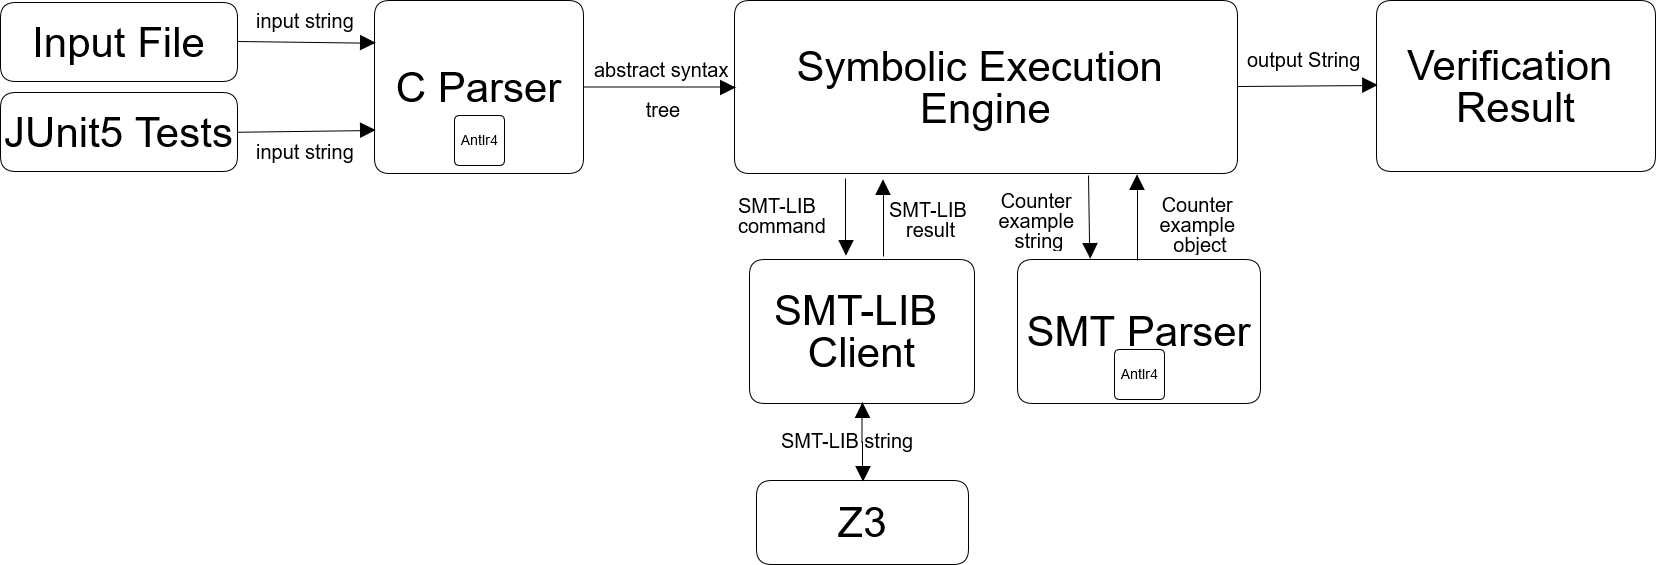
\includegraphics[scale=.21,keepaspectratio=true]{./engine.png}
\end{figure}
\end{frame}

%\definecolor{light-gray}{gray}{0.95}
%\lstset{backgroundcolor= \color{light-gray}}

\begin{frame}[fragile]
\frametitle{Execution}
\scriptsize

\begin{block}{Input: test.c}
\begin{lstlisting}  
void f (int x, int y)
{
    if(x > 0)
    {
        y = x;
    }
    assert (y == x);
}
\end{lstlisting}
\end{block}
\end{frame}


\begin{frame}[fragile]
\frametitle{Execution}
\begin{block} {Output: java -jar SymbolicEngine.jar -i test.c}
\small
\begin{lstlisting} 
------------------
Overall Answer: No
------------------
Assertion: (BinaryExpression(Variable(y) == Variable(x)))
AssertionFormula:
(assert (> _x1 0))
(assert (not (= _x1 _x1)))
Answer: Yes
----------------------------
AssertionFormula:
(assert (not (> _x1 0)))
(assert (not (= _x2 _x1)))
Answer: No
Counter example: {x=0, y=1}
----------------------------
\end{lstlisting} 
\end{block}
\end{frame}


\begin{frame}[fragile]
\frametitle{Execution}
\huge
\centering

Demo

\end{frame}

\begin{frame}[fragile]
\frametitle{Motivation or Importance of the problem}
\begin{block}{Importance of symbolic execution}
\begin{itemize}
\item Software verification for critical systems
\item Security properties: e.g. access array within boundaries
\item Safety properties: microwave should not run while its door is open
\end{itemize}
\end{block}

\begin{block}{Personal motivation}
\begin{itemize}
\item Related to my research 
\item A tedious question in the second midterm
\end{itemize}
\end{block}

\end{frame}

\begin{frame}[fragile]
\frametitle{Challenges}
\begin{block}{General challenges}
\begin{itemize}
\item Scalability
\item Memory
\item Environment
\item Loops
\item Solver limitations
\end{itemize}
\end{block}
\end{frame}

\begin{frame}[fragile]
\frametitle{Challenges}
\begin{block}{Project challenges}
\begin{itemize}
\item A grammar for C
\item A grammar for SMT-LIB
\item Deadlock with Z3 process

\end{itemize}
\end{block}
\end{frame}

\begin{frame}[fragile]
\frametitle{Existing approaches}
\begin{itemize}
\item Concolic execution
\item Dynamic symbolic execution
\item Selective symbolic execution
\item Path selection
\item Symbolic backward execution
\item Fully symbolic memory
\item Address concretization
\item Partial memory modeling
\item Lazy initialization

\end{itemize}
\end{frame}

\begin{frame}[fragile]
\frametitle{My approach}
\begin{itemize}
\item Only handles functions
\item Simple integer variables
\item No pointers, arrays, structs 
\item No bitwise operations
\item No loops
\item Fully symbolic execution
\end{itemize}
\end{frame}

\begin{frame}[fragile]
\frametitle{My approach}
\begin{itemize}
\item Start with function definition
\item Assign a new symbolic value to each argument variable
\item Set the initial path constraint to empty (i.e. $true$)
\item \textbf{Initial start state} = argument variables(with symbolic values) + empty constraint
\item Each statement has \textbf{start states} and \textbf{end states}. A statement can't modify its \textbf{start states}

\item The block of the function has one \textbf{start state} = \textbf{Initial start state}

\item The first statement in each block has the same \textbf{start states} of its block

\item Each subsequent statement has the same \textbf{start states} of the previous statement
\end{itemize}
\end{frame}


\begin{frame}[fragile]
\frametitle{My approach}
\begin{itemize}
\item An assignment statement ($variable = expression$) has \textbf{end states} exactly as \textbf{start states} except with the updated $variable$ which gets the symbolic value of the $expression$

\item A variable definition statement without assignment has \textbf{end states} exactly as \textbf{start states} except with the addition of the new variable which gets a new symbolic value

\begin{lstlisting}  
void f()
{
	int z;
	assert (z == z);
}
\end{lstlisting}

\item  A variable definition statement with assignment has \textbf{end states} exactly as \textbf{start states} except with the addition of the new variable which gets the value of the $expression$

\end{itemize}
\end{frame}

\begin{frame}[fragile]
\frametitle{My approach}
\begin{itemize}
\item Statements like (++i) or (i++) are rewritten as assignment statements (e.g. i = i + 1;)
\item \textbf{If statement} will add its condition to the path constraint of each start state of its
\textbf{true statement}. Likewise, the \textbf{If statement} will add the negation of its condition to the
path constraint of each start state of its \textbf{false statement}


\end{itemize}
\end{frame}


\begin{frame}[fragile]
\frametitle{My approach}
\begin{itemize}

\item If the \textbf{If statement} has no \textbf{false statement}, NoOperation statement will be used instead

\begin{lstlisting}  
void f (int x, int y) 
{ 
	if(x > 0) y = x;  
	assert (y == x);
}
\end{lstlisting}

\begin{lstlisting}  
void f (int x, int y) 
{ 
	if(x > 0) y = x;  
	else NoOperation();
	assert (y == x);
}
\end{lstlisting}

\end{itemize}
\end{frame}


\begin{frame}[fragile]
\frametitle{My approach}
\begin{itemize}

\item For each division operation, a new assertion statement would be added. The \textbf{start states} of this assertion would be the \textbf{start states} of the statement where the division resides

\begin{lstlisting}  
void f (int x, int y) 
{
	x = x / y;
}
\end{lstlisting}

\begin{lstlisting}  
void f (int x, int y) 
{
	assert(y != 0);
	x = x / y;
}
\end{lstlisting}

\end{itemize}
\end{frame}


\begin{frame}[fragile]
\frametitle{My approach}
\begin{itemize}

\item Integers as booleans

\begin{lstlisting}  
void f (int x, int y) 
{ 	
	assert (x+y);
	assert (0);
}
\end{lstlisting}

\begin{lstlisting}  
void f (int x, int y) 
{ 	
	assert (x+y > 0);
	assert (0 > 0);
}
\end{lstlisting}

\end{itemize}
\end{frame}


\begin{frame}[fragile]
\frametitle{My approach}
\begin{itemize}

\item Unknown

\begin{lstlisting}  
void f (int x, int y, int z)  +
{
	assert(!((x*x*x + y*y*y == z*z*z) && 
	(x>10) && (y>10) && (z>10)));
};
\end{lstlisting}


\end{itemize}
\end{frame}


\begin{frame}[fragile]
\frametitle{Work Division}
Since there is only one person in this project, all the work is done by him
\end{frame}

\begin{frame}[fragile]
\frametitle{References}
Roberto Baldoni, Emilio Coppa, Daniele Cono D’Elia, Camil Demetrescu, and Irene Finocchi.
A survey of symbolic execution techniques. CoRR, abs/1610.00502, 2016
\end{frame}


\end{document}
